\documentclass[aspectratio=169, table, 12pt]{beamer}

% Preamble bersama seluruh slide mata kuliah ini.
% Dipanggil dari slides/sessionXX/sessionXX.tex tepat sesudah baris
% \documentclass[aspectratio=169, table, 12pt]{beamer}
% Paket tambahan yang hanya dibutuhkan satu sesi ditulis di berkas sesi itu.

\usepackage{colortbl}
\usepackage{xcolor}
\usepackage{listings}
\usepackage{tabularx}
\usepackage{booktabs}
\usepackage{tikz}
\usepackage{pgfplots}
\pgfplotsset{compat=1.18}
\usetikzlibrary{arrows.meta, positioning, calc, fit, shapes.geometric,
	shapes.multipart, backgrounds, matrix, chains, trees}

\makeatletter
\def\input@path{{../theme/}}
\makeatother
\graphicspath{{../theme/}{../../figures/}}
\usetheme{Pradita}

\definecolor{praditagreen}{RGB}{37, 113, 71}

% Tema membuat garis tabel berwarna putih. Dikembalikan agar tabel terbaca.
\arrayrulecolor{black}
\setlength{\arrayrulewidth}{0.5pt}

\lstdefinelanguage{yaml}{
	basicstyle=\ttfamily\scriptsize,
	keywordstyle=\color{blue}\bfseries,
	commentstyle=\color{gray}\itshape,
	stringstyle=\color{red},
	showstringspaces=false,
	breaklines=true,
	frame=lines,
	numbers=none,
	backgroundcolor=\color{lightgray!10},
	tabsize=2,
	morecomment=[l]{\#}
}

\lstdefinelanguage{json}{
	basicstyle=\ttfamily\scriptsize,
	stringstyle=\color{red},
	commentstyle=\color{gray},
	breaklines=true,
	showstringspaces=false,
	tabsize=2,
	numbers=none,
	frame=lines,
	backgroundcolor=\color{lightgray!10},
	string=[s]{"}{"}
}

\lstdefinelanguage{bash}{
	keywords={},
	basicstyle=\ttfamily\scriptsize,
	ndkeywords={docker, kubectl, helm, curl, git, terraform},
	ndkeywordstyle=\color{purple}\bfseries,
	sensitive=true,
	commentstyle=\color{gray},
	numbers=none,
	breaklines=true,
	frame=lines,
	backgroundcolor=\color{lightgray!10},
	tabsize=2,
	comment=[l]{\#},
	showstringspaces=false
}

\lstdefinelanguage{http}{
	keywords={GET, POST, PUT, PATCH, DELETE, HEAD, OPTIONS, HTTP},
	basicstyle=\ttfamily\scriptsize,
	keywordstyle=\color{blue}\bfseries,
	sensitive=true,
	numbers=none,
	breaklines=true,
	frame=lines,
	backgroundcolor=\color{lightgray!10},
	tabsize=2,
	showstringspaces=false
}

\subtitle{IT40713 · Cloud-Native \& Microservices Architecture}
\author{\textbf{Alfa Yohannis}}


\title{\Huge Container, Kubernetes\\ \vspace{10pt} dan Serverless}

% Butir masalah dipakai pada slide dengan atau tanpa ilustrasi.
\newcommand{\chdelapanmasalah}{%
  \begin{itemize}
    \item Modul pendaftaran lancar di Jakarta, gagal di Bandung: versi
          pustaka berbeda.
    \item Tiga hari habis untuk menemukan penyebabnya.
    \item Skrip pengingat kontrol: server menyala 24 jam untuk kerja
          beberapa menit.
    \item Pertanyaannya: di mana dan dengan cara apa layanan dijalankan
          (\textit{runtime})?
  \end{itemize}}

\begin{document}

\frame{\titlepage}

\begin{frame}
  \frametitle{Isi Pertemuan}
  \vspace{14pt}
  \begin{columns}[t]
    \column{0.5\textwidth}
    {\small\tableofcontents[sections={1-4}]}

    \column{0.5\textwidth}
    {\small\tableofcontents[sections={5-8}]}
  \end{columns}
\end{frame}

\begin{frame}{\hfill}
  \centering
  \Huge{\textbf{Mengapa aplikasi yang\\lancar di Jakarta bisa\\gagal di Bandung?}}
\end{frame}

\section{Tujuan dan Konteks}

\begin{frame}{\hfill}
  \centering
  \Huge{\textbf{Tujuan dan Konteks}}
\end{frame}

\begin{frame}{{\Large Tujuan Pembelajaran}}
  \vspace{10pt}
  \begin{itemize}
    \item Menjelaskan perbedaan \textit{virtual machine}, \textit{container},
          dan \textit{serverless} dengan analogi dan contoh.
    \item Menjelaskan cara Kubernetes menjaga sistem tetap sesuai keadaan
          yang diinginkan.
    \item Memilih \textit{runtime} untuk setiap kandidat layanan berdasarkan
          kriteria yang eksplisit.
  \end{itemize}
\end{frame}

\begin{frame}{{\Large Diagram Konsep Bab 8}}
  \centering
  {\small\bfseries Kubernetes merekonsiliasi keadaan yang diinginkan}\par\medskip
  \adjustbox{width=0.96\textwidth,height=0.7\textheight,keepaspectratio}{%
    % Diagram konsep Bab 8: Kubernetes merekonsiliasi keadaan yang diinginkan.
% Dibangkitkan tools/render-diagrams.py dari figures/chapter-diagrams.json;
% ubah data JSON lalu jalankan ulang skrip, jangan sunting berkas ini langsung.
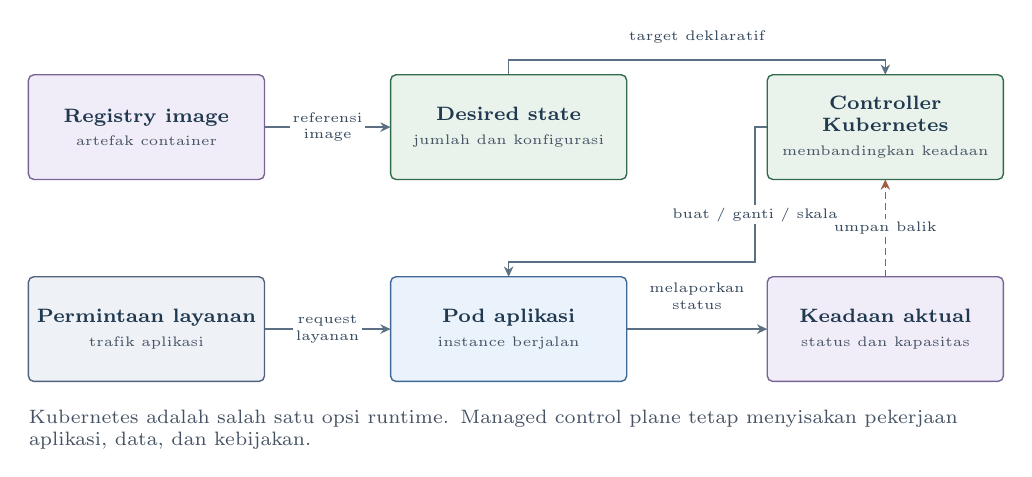
\begin{tikzpicture}[
  x=0.92cm, y=0.95cm,
  kotak konsep/.style={draw, line width=0.5pt, rounded corners=2pt,
    align=center, minimum width=2.999cm,
    minimum height=1.330cm, inner sep=0pt, font=\scriptsize,
    text=konsepJudul},
  peran actor/.style={kotak konsep, fill=konsepIsiActor, draw=konsepGarisActor},
  peran service/.style={kotak konsep, fill=konsepIsiService, draw=konsepGarisService},
  peran control/.style={kotak konsep, fill=konsepIsiControl, draw=konsepGarisControl},
  peran data/.style={kotak konsep, fill=konsepIsiData, draw=konsepGarisData},
  peran outcome/.style={kotak konsep, fill=konsepIsiOutcome, draw=konsepGarisOutcome},
  peran risk/.style={kotak konsep, fill=konsepIsiRisk, draw=konsepGarisRisk},
  panah konsep/.style={-{Stealth[length=1.3mm, width=1.2mm]}, line width=0.6pt,
    draw=konsepPanah},
  panah putus/.style={panah konsep, draw=konsepPanahPutus,
    dash pattern=on 2.5pt off 1.5pt},
  label panah/.style={font=\tiny, align=center, fill=white,
    inner sep=1pt, text=konsepLabel},
  catatan/.style={font=\scriptsize, align=left, anchor=north west,
    inner sep=0pt, text width=12.383cm, text=konsepTeks,
    execute at begin node={\hyphenpenalty=10000\hbadness=10000\relax}},
]
  \definecolor{konsepIsiActor}{HTML}{EEF1F6}
  \definecolor{konsepGarisActor}{HTML}{50627D}
  \definecolor{konsepIsiService}{HTML}{EAF2FB}
  \definecolor{konsepGarisService}{HTML}{3F6893}
  \definecolor{konsepIsiControl}{HTML}{E9F3EC}
  \definecolor{konsepGarisControl}{HTML}{316B4B}
  \definecolor{konsepIsiData}{HTML}{F1EDF8}
  \definecolor{konsepGarisData}{HTML}{786394}
  \definecolor{konsepIsiOutcome}{HTML}{E4F2EC}
  \definecolor{konsepGarisOutcome}{HTML}{236C57}
  \definecolor{konsepIsiRisk}{HTML}{FCEDE7}
  \definecolor{konsepGarisRisk}{HTML}{B36947}
  \definecolor{konsepJudul}{HTML}{20394F}
  \definecolor{konsepTeks}{HTML}{455264}
  \definecolor{konsepLabel}{HTML}{35485C}
  \definecolor{konsepPanah}{HTML}{5C7084}
  \definecolor{konsepPanahPutus}{HTML}{A15D40}
  % Panah dan label lebih dahulu; kotak menutupi sisa latar label.
  \draw[panah konsep] (0.93,0) -- (2.67,0);
  \draw[panah konsep] (4.3,0.7) -- (4.3,0.9) -- (9.5,0.9) -- (9.5,0.7);
  \draw[panah konsep] (7.87,0) -- (7.7,0) -- (7.7,-1.8) -- (4.3,-1.8) -- (4.3,-2);
  \draw[panah konsep] (5.93,-2.7) -- (7.87,-2.7);
  \draw[panah putus] (9.5,-2) -- (9.5,-0.7);
  \draw[panah konsep] (0.93,-2.7) -- (2.67,-2.7);
  \node[label panah] at (1.8,0) {referensi\\image};
  \node[label panah] at (6.9,1.21) {target deklaratif};
  \node[label panah] at (7.7,-1.17) {buat / ganti / skala};
  \node[label panah] at (6.9,-2.26) {melaporkan\\status};
  \node[label panah] at (9.5,-1.35) {umpan balik};
  \node[label panah] at (1.8,-2.7) {request\\layanan};
  \node[peran data] (artefak) at (-0.7,0)
    {\textbf{Registry image}\\[0.5pt]{\tiny\color{konsepTeks}artefak container}};
  \node[peran control] (desired) at (4.3,0)
    {\textbf{Desired state}\\[0.5pt]{\tiny\color{konsepTeks}jumlah dan konfigurasi}};
  \node[peran control] (controller) at (9.5,0)
    {\textbf{Controller}\\\textbf{Kubernetes}\\[0.5pt]{\tiny\color{konsepTeks}membandingkan keadaan}};
  \node[peran actor] (pengguna) at (-0.7,-2.7)
    {\textbf{Permintaan layanan}\\[0.5pt]{\tiny\color{konsepTeks}trafik aplikasi}};
  \node[peran service] (pod) at (4.3,-2.7)
    {\textbf{Pod aplikasi}\\[0.5pt]{\tiny\color{konsepTeks}instance berjalan}};
  \node[peran data] (actual) at (9.5,-2.7)
    {\textbf{Keadaan aktual}\\[0.5pt]{\tiny\color{konsepTeks}status dan kapasitas}};
  \node[catatan] at (-2.33,-3.77)
    {Kubernetes adalah salah satu opsi runtime. Managed control plane tetap menyisakan pekerjaan aplikasi, data, dan kebijakan.};
\end{tikzpicture}
}
\end{frame}

\section{VM dan Container}

\begin{frame}{\hfill}
  \centering
  \Huge{\textbf{Virtual Machine\\dan Container}}
\end{frame}

\begin{frame}{{\Large Virtual Machine dan Container}}
  \vspace{6pt}
  \begin{itemize}
    \item VM: komputer tiruan di atas \textit{hypervisor}, membawa sistem
          operasi tamu sendiri.
    \item \textit{Container}: aplikasi dan pustakanya, berjalan sebagai proses
          terisolasi, berbagi satu \textit{kernel} host.
    \item \textit{Container} lebih kecil dan cepat menyala; VM lebih berat,
          isolasinya lebih tebal.
    \item Analogi: peti kemas standar. Isinya berbeda, cara mengangkutnya
          sama.
  \end{itemize}
\end{frame}

\begin{frame}{{\Large Susunan Lapisan VM dan Container}}
  \centering
  \eadiagram{../../figures/ch08-vm-container.tex}
\end{frame}

\begin{frame}{{\Large Dua Contoh dari Medikara Health}}
  \vspace{6pt}
  \begin{itemize}
    \item Modul pendaftaran dikemas sebagai \textit{container} bersama pustaka
          yang sudah diuji; kemasan sama dipakai di lima rumah sakit.
    \item Misalkan rumah sakit Depok menjalankan 12 aplikasi kecil, satu VM
          per aplikasi.
    \item Sekitar 2 GB memori per sistem operasi tamu: 24 GB habis hanya
          untuk sistem operasi.
    \item Sebagai \textit{container} di dua host: sistem operasi yang dirawat
          tinggal dua.
  \end{itemize}
\end{frame}

\begin{frame}{{\Large Container Image dan Registry}}
  \footnotesize
  \begin{tabularx}{\textwidth}{>{\raggedright\arraybackslash}p{2.6cm}
      >{\raggedright\arraybackslash}X >{\raggedright\arraybackslash}X}
    \hline
    \textbf{Istilah} & \textbf{Arti} & \textbf{Contoh} \\
    \hline
    \textit{Container image} & Paket baca-saja, aplikasi dan dependensinya &
      \texttt{jadwal-dokter:1.4.2} \\
    \hline
    \textit{Container} & \textit{Image} yang sedang berjalan & Tiga
      \textit{container} di rumah sakit Bandung \\
    \hline
    \textit{Registry} & Gudang \textit{image} & \textit{Registry} privat di
      \textit{region} Jakarta \\
    \hline
    \textit{Tag} dan \textit{digest} & Nama versi dan sidik jari isi &
      Produksi memakai \textit{digest} yang sudah diuji \\
    \hline
  \end{tabularx}

  \vspace{8pt}
  \small
  Format \textit{image} distandarkan Open Container Initiative.
  \textit{Registry} menjadi aset kritis, dan \textit{image} tidak boleh
  memuat data pasien.
\end{frame}

\begin{frame}{{\Large Batas Isolasi Container}}
  \footnotesize
  \begin{tabularx}{\textwidth}{>{\raggedright\arraybackslash}p{2.6cm}
      >{\raggedright\arraybackslash}X >{\raggedright\arraybackslash}X}
    \hline
    \textbf{Aspek} & \textbf{\textit{Virtual machine}} &
      \textbf{\textit{Container}} \\
    \hline
    Batas isolasi & \textit{Kernel} sendiri & Berbagi satu \textit{kernel} \\
    \hline
    Waktu menyala & Lebih lama & Cepat \\
    \hline
    Cocok untuk & Aplikasi lama, isolasi ketat & Layanan baru yang sering
      diperbarui \\
    \hline
  \end{tabularx}

  \vspace{6pt}
  \small
  \begin{itemize}
    \item NIST SP 800-190: kelompokkan \textit{container} menurut tujuan dan
          sensitivitas.
    \item Medikara: \textit{container} Medikara+ tidak satu host dengan
          pengolah rekam medis.
  \end{itemize}
\end{frame}

\section{Kubernetes}

\begin{frame}{\hfill}
  \centering
  \Huge{\textbf{Orkestrasi Container\\dan Kubernetes}}
\end{frame}

\begin{frame}{{\Large Mengapa Perlu Orkestrasi}}
  \vspace{6pt}
  \begin{itemize}
    \item Misalkan 9 layanan, 3 replika, 3 lingkungan: 81 \textit{container}.
    \item Server mana yang masih punya ruang?
    \item Siapa menyalakan ulang \textit{container} yang mati pukul 02.00?
    \item Bagaimana memasang versi baru tanpa menghentikan layanan?
    \item Siapa menambah kapasitas pukul 07.00?
  \end{itemize}
  \vspace{4pt}
  {\small Kubernetes: orkestrator \textit{open source}, lahir dari pengalaman
  Google dengan Borg dan Omega.}
\end{frame}

\begin{frame}{{\Large Desired State dan Rekonsiliasi}}
  \vspace{6pt}
  \begin{itemize}
    \item Tim menulis keadaan yang diinginkan di manifest: "tiga replika
          versi 1.4.2".
    \item Kontroler: lingkaran kendali yang mengamati, membandingkan, lalu
          bertindak.
    \item Analogi: kepala ruang perawat menjaga angka "enam perawat per sif".
    \item Konsekuensi 1: keadaan sistem dapat diaudit dari manifest.
    \item Konsekuensi 2: perubahan manual di klaster dikembalikan kontroler.
  \end{itemize}
\end{frame}

\begin{frame}{{\Large Satu Putaran Rekonsiliasi}}
  \centering
  \eadiagram{../../figures/ch08-rekonsiliasi.tex}
\end{frame}

\begin{frame}{{\Large Pod, Deployment, dan Service}}
  \footnotesize
  \begin{tabularx}{\textwidth}{>{\raggedright\arraybackslash}p{2.6cm}
      >{\raggedright\arraybackslash}X >{\raggedright\arraybackslash}X}
    \hline
    \textbf{Konsep} & \textbf{Fungsi} & \textbf{Contoh Medikara} \\
    \hline
    Klaster dan \textit{node} & Sekumpulan server yang dikelola sebagai satu &
      Enam \textit{node} di \textit{region} Jakarta \\
    \hline
    \textit{Control plane} & Menyimpan keadaan, menjadwalkan, menjalankan
      kontroler & Diurus penyedia pada \textit{managed} Kubernetes \\
    \hline
    \textit{Pod} & Unit terkecil, satu atau beberapa \textit{container} & Satu
      \textit{pod} jadwal dokter \\
    \hline
    \textit{Deployment} & Jumlah replika dan versi \textit{image} & Tiga replika
      \texttt{jadwal-dokter:1.4.2} \\
    \hline
    \textit{Service} & Alamat tetap untuk \textit{pod} yang berganti &
      Dipanggil layanan janji temu \\
    \hline
  \end{tabularx}
\end{frame}

\begin{frame}{{\Large Self-Healing dan Autoscaling}}
  \vspace{6pt}
  \begin{itemize}
    \item \textit{Self-healing}: \textit{container} gagal dinyalakan ulang,
          \textit{pod} di \textit{node} mati diganti.
    \item Misalkan \textit{node} mati pukul 02.10: \textit{pod} pengganti
          muncul dalam sekitar satu menit.
    \item \textit{Autoscaling}: replika ditambah atau dikurangi menurut beban.
    \item Janji temu: 10 menjadi 50 permintaan per detik pukul 07.00 sampai
          09.00, termasuk pengecekan jadwal dan kuota.
    \item Target prosesor 70 persen, tiga sampai delapan replika.
  \end{itemize}
\end{frame}

\begin{frame}{{\Large Membaca Survei CNCF 2025}}
  \footnotesize
  \begin{tabularx}{\textwidth}{>{\raggedright\arraybackslash}X
      >{\raggedright\arraybackslash}p{2.4cm} >{\raggedright\arraybackslash}X}
    \hline
    \textbf{Indikator} & \textbf{Angka} & \textbf{Cara membaca} \\
    \hline
    Responden dan waktu survei & 628, September 2025 & Sampel komunitas, bukan
      sensus \\
    \hline
    Pengguna \textit{container} yang menjalankan Kubernetes di produksi &
      82 persen (2023: 66 persen) & Penyebutnya pengguna \textit{container} \\
    \hline
    Organisasi dengan model AI generatif sendiri yang memakai Kubernetes
      untuk inferensi & 66 persen & Penyebutnya organisasi yang menjalankan
      model sendiri \\
    \hline
  \end{tabularx}

  \vspace{8pt}
  \small
  Ekosistemnya besar, tetapi angka adopsi tidak menjawab apakah Kubernetes
  tepat untuk tim kecil.
\end{frame}

\section{Managed Kubernetes dan PaaS}

\begin{frame}{\hfill}
  \centering
  \Huge{\textbf{Managed Kubernetes\\dan PaaS}}
\end{frame}

\begin{frame}{{\Large Managed Kubernetes dan PaaS}}
  \vspace{6pt}
  \begin{itemize}
    \item \textit{Managed} Kubernetes: penyedia menjalankan \textit{control
          plane}.
    \item Pelanggan tetap mengurus manifest, \textit{image}, izin akses,
          jaringan, dan pembaruan \textit{node}.
    \item PaaS: serahkan kode atau \textit{image}; platform mengurus server,
          \textit{runtime}, dan skala.
    \item \textit{Managed} Kubernetes memperlihatkan Kubernetes; PaaS
          menyembunyikannya.
    \item Analogi: dapur sendiri, sewa dapur komersial, katering.
  \end{itemize}
\end{frame}

\begin{frame}{{\Large Pembagian Tanggung Jawab}}
  \centering
  \eadiagram{../../figures/ch08-spektrum-tanggung-jawab.tex}
\end{frame}

\begin{frame}{{\Large Biaya Control Plane dan Irama Pembaruan}}
  \vspace{6pt}
  \begin{itemize}
    \item AWS: 0,10 dolar AS per klaster per jam (dukungan standar), 0,60
          dolar AS (diperpanjang).
    \item Tiga klaster: 219 dolar AS per bulan, sekitar Rp3,6 juta (kurs
          asumsi Rp16.500).
    \item Terlambat memperbarui: 1.314 dolar AS, sekitar Rp21,7 juta per
          bulan.
    \item Kubernetes: sekitar tiga rilis minor per tahun, dukungan
          \textit{patch} sekitar satu tahun.
    \item Misalkan tiga pembaruan per klaster per tahun: 90 hari kerja.
  \end{itemize}
\end{frame}

\begin{frame}{{\Large Kasus Medikara: Biaya Tiga Opsi}}
  \scriptsize
  \begin{tabularx}{\textwidth}{>{\raggedright\arraybackslash}X r r r}
    \hline
    \textbf{Komponen (juta rupiah per tahun)} & \textbf{Sendiri} &
      \textbf{\textit{Managed}} & \textbf{PaaS} \\
    \hline
    \textit{Control plane} & 180 & 43 & 0 \\
    \hline
    Kapasitas komputasi sembilan layanan & 600 & 600 & 720 \\
    \hline
    Tenaga kerja platform (jumlah orang) & 1.560 (4) & 780 (2) & 390 (1) \\
    \hline
    Pelatihan, alat pemantauan, dan keamanan & 270 & 240 & 90 \\
    \hline
    \textbf{Total satu tahun} & \textbf{2.610} & \textbf{1.663} &
      \textbf{1.200} \\
    \hline
  \end{tabularx}

  \vspace{8pt}
  \small
  \begin{itemize}
    \item Tenaga kerja 46,9 persen biaya \textit{managed}; \textit{control
          plane} hanya 2,6 persen.
    \item Usulan: PaaS untuk layanan baru pertama, hemat Rp463 juta (27,8
          persen).
  \end{itemize}
\end{frame}

\section{Serverless}

\begin{frame}{\hfill}
  \centering
  \Huge{\textbf{Serverless dan\\Function as a Service}}
\end{frame}

\begin{frame}{{\Large Serverless dan FaaS}}
  \vspace{6pt}
  \begin{itemize}
    \item Server diurus penuh penyedia; kapasitas otomatis, menyusut sampai
          nol.
    \item Tagihan mengikuti pemakaian nyata, per eksekusi.
    \item FaaS: fungsi kecil yang dijalankan setiap kali ada pemicu.
    \item Kajian Berkeley: \textit{serverless} adalah FaaS ditambah
          \textit{Backend as a Service}.
    \item Analogi: lampu sensor gerak di lorong kantor.
  \end{itemize}
\end{frame}

\begin{frame}{{\Large Alur Function as a Service}}
  \centering
  \eadiagram{../../figures/ch08-alur-serverless.tex}
\end{frame}

\begin{frame}{{\Large Biaya per Eksekusi dan Keterbatasan}}
  \vspace{6pt}
  \begin{itemize}
    \item AWS Lambda: 0,20 dolar AS per satu juta permintaan dan
          0,0000166667 dolar AS per GB-detik (x86, AS Timur).
    \item Kuota gratis per bulan: satu juta permintaan dan 400.000 GB-detik.
    \item \textit{Cold start}: permintaan pertama setelah sepi menunggu lebih
          lama.
    \item Batas waktu: AWS Lambda paling lama 900 detik (15 menit).
    \item Ketergantungan: format pemicu, \textit{event}, dan izin akses khas
          penyedia.
  \end{itemize}
\end{frame}

\begin{frame}{{\Large Pola Beban yang Cocok}}
  \scriptsize
  \begin{tabularx}{\textwidth}{>{\raggedright\arraybackslash}p{3.2cm}
      >{\raggedright\arraybackslash}X >{\raggedright\arraybackslash}p{3.2cm}}
    \hline
    \textbf{Pola beban} & \textbf{Contoh Medikara} & \textbf{Kecocokan} \\
    \hline
    Jarang, tidak menentu & Ekspor data untuk auditor & Sangat cocok \\
    \hline
    Berkala terjadwal & Pengingat kontrol 06.00 dan 18.00 & Cocok \\
    \hline
    Dipicu kedatangan data & Hasil laboratorium tiap 30 menit & Cocok, dengan
      syarat \\
    \hline
    Lonjakan tajam singkat & Pendaftaran kampanye vaksinasi & Cocok, dengan
      catatan \\
    \hline
    Tinggi dan stabil 24 jam & Antarmuka SIMRS rawat inap & Kurang cocok \\
    \hline
    Proses panjang & Rekonsiliasi klaim bulanan tiga jam & Tidak cocok tanpa
      dipecah \\
    \hline
  \end{tabularx}
\end{frame}

\begin{frame}{{\Large Kasus Medikara: Pengingat Jadwal Kontrol}}
  \vspace{6pt}
  \begin{itemize}
    \item Misalkan 40 persen dari 1,2 juta kunjungan: 40.000 jadwal kontrol
          per bulan.
    \item Dua pengingat: 80.000 eksekusi, 0,5 detik, 0,25 GB: 10.000
          GB-detik.
    \item \textit{Serverless} sekitar Rp3.000 per bulan tanpa kuota gratis;
          VM Rp650.000, pemanfaatan sekitar 1,5 persen.
    \item Biaya pesan WhatsApp Rp28 juta per bulan, apa pun
          \textit{runtime}-nya.
    \item Argumen utama: tanpa \textit{patch} server, kapasitas menyesuaikan
          sendiri.
  \end{itemize}
\end{frame}

\begin{frame}{{\Large Kasus Medikara: Hasil Laboratorium}}
  \vspace{6pt}
  \begin{itemize}
    \item 32 berkas per hari, sekitar 150 hasil per berkas.
    \item Desain awal: satu fungsi terjadwal memproses semua berkas yang
          menunggu.
    \item Sistem laboratorium mati lima jam: 10 berkas, 20 menit, melampaui
          batas 15 menit.
    \item Perbaikan: fungsi pemecah per berkas, lalu satu hasil per eksekusi.
    \item Fungsi, antrean, dan penyimpanan di \textit{region} Jakarta
          (matriks Bab 2).
  \end{itemize}
\end{frame}

\section{Memilih Runtime}

\begin{frame}{\hfill}
  \centering
  \Huge{\textbf{Memilih Runtime dan\\Vendor Lock-in}}
\end{frame}

\begin{frame}{{\Large Kriteria Memilih Runtime}}
  \scriptsize
  \begin{tabularx}{\textwidth}{>{\raggedright\arraybackslash}p{3.6cm}
      >{\raggedright\arraybackslash}X >{\raggedright\arraybackslash}p{1.2cm}}
    \hline
    \textbf{Kriteria} & \textbf{Pertanyaan kunci} & \textbf{Bobot} \\
    \hline
    Lokasi data & Tersedia di lokasi yang diizinkan (Bab 2)? & Gugur \\
    \hline
    Kecocokan pola beban & Kapan dan seberapa sering dipakai? & 25 \\
    \hline
    Kebutuhan latensi & Adakah orang yang menunggu jawaban? & 15 \\
    \hline
    Keterampilan tim dan pasar & Siapa yang mengoperasikan pukul 02.00? & 25 \\
    \hline
    Biaya total tiga tahun & Termasuk tenaga kerja dan biaya keluar? & 20 \\
    \hline
    Portabilitas dan \textit{lock-in} & Berapa upaya pindah penyedia? & 15 \\
    \hline
  \end{tabularx}

  \vspace{6pt}
  \small
  Kriteria dan bobot ditulis sebelum opsi mana pun dinilai.
\end{frame}

\begin{frame}{{\Large Matriks Keputusan: Layanan Janji Temu}}
  \scriptsize
  \begin{tabularx}{\textwidth}{>{\raggedright\arraybackslash}X r r r r r r}
    \hline
    \textbf{Kriteria} & \textbf{Bobot} & \textbf{SaaS} & \textbf{PaaS} &
      \textbf{\textit{Managed}} & \textbf{\textit{Serverless}} & \textbf{VM} \\
    \hline
    Lokasi data & & Gugur & Lolos & Lolos & Lolos & Lolos \\
    \hline
    Pola beban & 25 & & 4 & 5 & 4 & 2 \\
    \hline
    Latensi & 15 & & 4 & 5 & 3 & 4 \\
    \hline
    Keterampilan tim & 25 & & 5 & 2 & 4 & 4 \\
    \hline
    Biaya total & 20 & & 4 & 2 & 4 & 3 \\
    \hline
    Portabilitas & 15 & & 3 & 4 & 2 & 4 \\
    \hline
    \textbf{Nilai berbobot} & & \textbf{-} & \textbf{4,10} & \textbf{3,50} &
      \textbf{3,55} & \textbf{3,30} \\
    \hline
  \end{tabularx}

  \vspace{6pt}
  \small
  Keterampilan \textit{managed} naik ke 4: nilainya 4,00. Pengingat kontrol:
  \textit{serverless} 4,45, VM 3,00.
\end{frame}

\begin{frame}{{\Large Vendor Lock-in dan Biaya Keluar}}
  \vspace{6pt}
  \begin{itemize}
    \item Pindah penyedia menjadi mahal karena teknologi, format data, atau
          kontrak.
    \item Biaya keluar: transfer data keluar, penulisan ulang, pelatihan,
          operasi paralel.
    \item Misalkan 40 fungsi, 25 dengan pemicu khas: sekitar 75 hari kerja.
    \item \textit{Managed} Kubernetes: 12 dari 60 manifest khas, ditambah
          \textit{registry} dan izin: sekitar 16 hari kerja.
    \item \textit{Lock-in} boleh, asal disadari, dihitung, dan punya rencana
          keluar.
  \end{itemize}
\end{frame}

\section{Aktivitas}

\begin{frame}{{\Large Aktivitas: Matriks Keputusan Runtime}}
  \vspace{6pt}
  \begin{enumerate}
    \item Ambil kandidat layanan dari Bab 6 dan Bab 7.
    \item Tetapkan kriteria dan bobotnya sebelum menilai.
    \item Terapkan kriteria gugur lokasi data, lalu nilai SaaS, PaaS,
          \textit{managed} Kubernetes, \textit{serverless}, dan VM.
    \item Pilih \textit{runtime} dan catat alasannya dalam ADR singkat.
  \end{enumerate}
  \vspace{4pt}
  {\small Luaran: matriks keputusan \textit{runtime} per layanan untuk C3.}
\end{frame}

\begin{frame}{{\Large Peran dan Berkas Pendukung}}
  \vspace{6pt}
  \begin{itemize}
    \item Anggota teknis: konsekuensi operasional setiap opsi.
    \item Anggota non-teknis: biaya, pasar tenaga kerja, risiko
          ketergantungan.
    \item Seluruh anggota: menyepakati bobot sebelum penilaian.
    \item \berkas{sources/chapter08/matriks-keputusan-runtime.xlsx}
    \item Opsional: \berkas{sources/chapter08/contoh-container/} di klaster
          kind.
  \end{itemize}
\end{frame}

\section{Ringkasan dan Latihan}

\begin{frame}{{\Large Ringkasan}}
  \vspace{6pt}
  \begin{itemize}
    \item \textit{Container} membawa lingkungannya sendiri; bukan VM kecil.
    \item Kubernetes menjaga \textit{desired state} lewat rekonsiliasi.
    \item Kubernetes memindahkan pekerjaan operasi, tidak menghapusnya.
    \item \textit{Serverless} cocok untuk beban jarang, berkala, atau dipicu
          data.
    \item \textit{Runtime} yang tepat sanggup dijalankan tim yang ada, dengan
          rencana keluar tertulis.
  \end{itemize}
\end{frame}

\begin{frame}{{\Large Latihan}}
  \vspace{6pt}
  \begin{enumerate}
    \item Jelaskan kepada direktur keuangan mengapa layanan pengingat jadwal
          kontrol pasien cocok dijalankan secara \textit{serverless}.
    \item Kapan Kubernetes justru menjadi beban bagi organisasi? Berikan dua
          kondisi beserta alasannya.
    \item Bandingkan risiko \textit{vendor lock-in} pada layanan
          \textit{serverless} dan pada \textit{managed} Kubernetes.
  \end{enumerate}
\end{frame}

\end{document}
